\documentclass{article}
\usepackage{tikz}
\usepackage{float}
\usepackage{amsmath}
\usepackage{lmodern}
\usepackage{amssymb}
\usetikzlibrary{calc}
\usetikzlibrary{hobby}
\usetikzlibrary{decorations.markings}
\usetikzlibrary{patterns, patterns.meta}
\usetikzlibrary{shapes}
\usepackage{pgfplots}
\tikzset{
    cross/.style={cross out, draw=red, fill=none, minimum size=2*(#1-\pgflinewidth), inner sep=0pt, outer sep=0pt,line width = 0.8pt}, cross/.default={2.8pt},
  % style to apply some styles to each segment of a path
  on each segment/.style={
    decorate,
    decoration={
      show path construction,
      moveto code={},
      lineto code={
        \path [#1]
        (\tikzinputsegmentfirst) -- (\tikzinputsegmentlast);
      },
      curveto code={
        \path [#1] (\tikzinputsegmentfirst)
        .. controls
        (\tikzinputsegmentsupporta) and (\tikzinputsegmentsupportb)
        ..
        (\tikzinputsegmentlast);
      },
      closepath code={
        \path [#1]
        (\tikzinputsegmentfirst) -- (\tikzinputsegmentlast);
      },
    },
  },
  % style to add an arrow in the middle of a path
  mid arrow/.style={postaction={decorate,decoration={
        markings,
        mark=at position .5 with {\arrow[#1]{stealth}}
      }}},
}
\tikzset{arrowstyle/.style={->, >=stealth}}
\pgfplotsset{compat=1.18}
\begin{document}
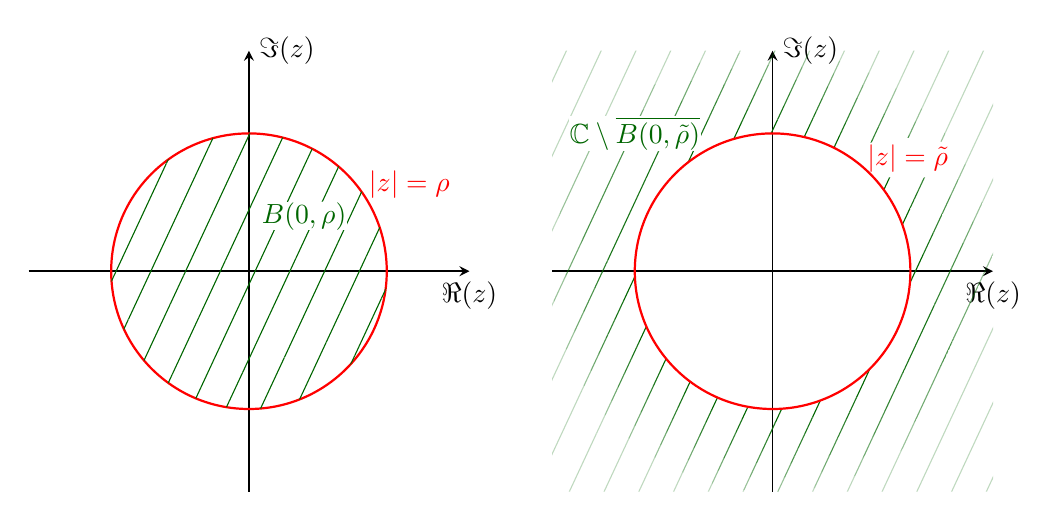
\begin{tikzpicture}[scale=0.7]
    \begin{scope}
      % draw axes
      \coordinate (O) at (0,0);
      \draw[arrowstyle, semithick] (0,-4) -- (0,4) node[anchor=west] {$\Im(z)$};
      \draw[arrowstyle, semithick] (-4,0) -- (4,0) node[anchor=north] {$\Re(z)$};

      % draw areas
      \draw[red, thick](2.5,0) arc[start angle=0, end angle=-360, radius=2.5];
      \fill[pattern={Lines[angle=65, distance=0.4cm]}, pattern color = black!60!green] (0,0) circle (2.5);

      \draw (2, 2) node[below right] {\textcolor{red}{$|z| = \rho$}};
      \node at (1,1) [draw=white, inner sep=0, fill=white] {\textcolor{black!60!green}{$B(0,\rho)$}};
    \end{scope}

    \begin{scope}[xshift=9.5cm]
    % draw axes
    \coordinate (O) at (0,0);
      \draw[arrowstyle, semithick] (0,-4) -- (0,4) node[anchor=west] {$\Im(z)$};
      \draw[arrowstyle, semithick] (-4,0) -- (4,0) node[anchor=north] {$\Re(z)$};

      % draw areas (change opacity to have a gradient fade)
      \fill[even odd rule, pattern={Lines[angle=65, distance=0.4cm]}, pattern color = black!60!green] (0,0) circle (2.5) circle (2.75);
      \fill[even odd rule, pattern={Lines[angle=65, distance=0.4cm]}, pattern color = black!60!green,opacity=0.9] (0,0) circle (2.75) circle (3);
      \fill[even odd rule, pattern={Lines[angle=65, distance=0.4cm]}, pattern color = black!60!green,opacity=0.8] (0,0) circle (3) circle (3.25);
      \fill[even odd rule, pattern={Lines[angle=65, distance=0.4cm]}, pattern color = black!60!green,opacity=0.7] (0,0) circle (3.25) circle (3.5);
      \fill[even odd rule, pattern={Lines[angle=65, distance=0.4cm]}, pattern color = black!60!green,opacity=0.55] (0,0) circle (3.5) circle (3.75);
      \fill[even odd rule, pattern={Lines[angle=65, distance=0.4cm]}, pattern color = black!60!green,opacity=0.4] (0,0) circle (3.75) circle (4);
      \fill[even odd rule, pattern={Lines[angle=65, distance=0.4cm]}, pattern color = black!60!green,opacity=0.25] (0,0) circle (4) (-4,4) rectangle (4,-4);

      % labels
      % \draw (2, 2) node[below right] {\textcolor{red}{$|z| = z_0$}};
      \node at (-2.5,2.5) [draw=white, inner sep=0, fill=white] {\textcolor{black!60!green}{$\mathbb{C} \setminus \overline{B(0,\tilde \rho)}$}};
      \node at (2.45,2.05) [draw=white, inner sep=0, fill=white, shape=ellipse] {\textcolor{red}{$|z| = \tilde \rho$}};
      % draw outline circle
      \draw[red, thick](2.5,0) arc[start angle=0, end angle=-360, radius=2.5];
    \end{scope}
\end{tikzpicture}

\end{document}